% Created by tikzDevice version 0.12.3.1 on 2022-09-02 16:28:59
% !TEX encoding = UTF-8 Unicode
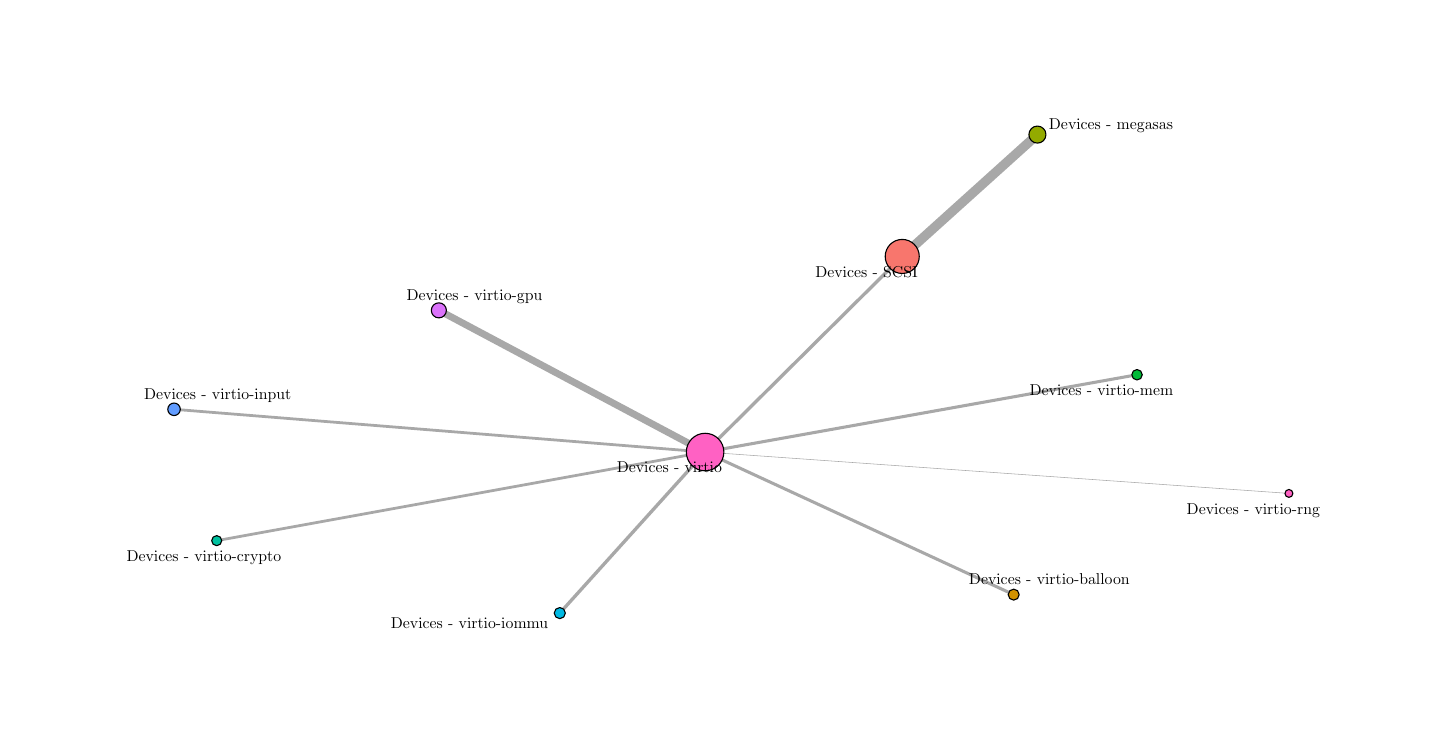
\begin{tikzpicture}[x=1pt,y=1pt]
\definecolor{fillColor}{RGB}{255,255,255}
\path[use as bounding box,fill=fillColor,fill opacity=0.00] (0,0) rectangle (505.89,252.94);
\begin{scope}
\path[clip] (  0.00,  0.00) rectangle (505.89,252.94);
\definecolor{fillColor}{RGB}{255,255,255}

\path[fill=fillColor] (  0.00,  0.00) rectangle (505.89,252.94);
\end{scope}
\begin{scope}
\path[clip] ( 32.75, 32.75) rectangle (475.89,222.94);
\definecolor{drawColor}{gray}{0.66}

\path[draw=drawColor,line width= 3.4pt,line join=round] (316.02,170.27) -- (364.87,214.30);

\path[draw=drawColor,line width= 1.2pt,line join=round] (316.02,170.27) -- (244.79, 99.59);

\path[draw=drawColor,line width= 1.1pt,line join=round] (244.79, 99.59) -- (356.29, 48.07);

\path[draw=drawColor,line width= 1.0pt,line join=round] (244.79, 99.59) -- ( 68.31, 67.57);

\path[draw=drawColor,line width= 2.5pt,line join=round] (244.79, 99.59) -- (148.58,150.79);

\path[draw=drawColor,line width= 1.0pt,line join=round] (244.79, 99.59) -- ( 52.89,115.04);

\path[draw=drawColor,line width= 1.2pt,line join=round] (244.79, 99.59) -- (192.28, 41.40);

\path[draw=drawColor,line width= 1.1pt,line join=round] (244.79, 99.59) -- (400.86,127.52);

\path[draw=drawColor,line width= 0.2pt,line join=round] (244.79, 99.59) -- (455.75, 84.64);
\definecolor{drawColor}{RGB}{0,0,0}
\definecolor{fillColor}{RGB}{248,118,109}

\path[draw=drawColor,line width= 0.4pt,line join=round,line cap=round,fill=fillColor] (316.02,170.27) circle (  6.15);
\definecolor{fillColor}{RGB}{147,170,0}

\path[draw=drawColor,line width= 0.4pt,line join=round,line cap=round,fill=fillColor] (364.87,214.30) circle (  3.08);
\definecolor{fillColor}{RGB}{255,97,195}

\path[draw=drawColor,line width= 0.4pt,line join=round,line cap=round,fill=fillColor] (244.79, 99.59) circle (  6.78);
\definecolor{fillColor}{RGB}{211,146,0}

\path[draw=drawColor,line width= 0.4pt,line join=round,line cap=round,fill=fillColor] (356.29, 48.07) circle (  1.99);
\definecolor{fillColor}{RGB}{0,193,159}

\path[draw=drawColor,line width= 0.4pt,line join=round,line cap=round,fill=fillColor] ( 68.31, 67.57) circle (  1.82);
\definecolor{fillColor}{RGB}{219,114,251}

\path[draw=drawColor,line width= 0.4pt,line join=round,line cap=round,fill=fillColor] (148.58,150.79) circle (  2.72);
\definecolor{fillColor}{RGB}{97,156,255}

\path[draw=drawColor,line width= 0.4pt,line join=round,line cap=round,fill=fillColor] ( 52.89,115.04) circle (  2.26);
\definecolor{fillColor}{RGB}{0,185,227}

\path[draw=drawColor,line width= 0.4pt,line join=round,line cap=round,fill=fillColor] (192.28, 41.40) circle (  2.01);
\definecolor{fillColor}{RGB}{0,186,56}

\path[draw=drawColor,line width= 0.4pt,line join=round,line cap=round,fill=fillColor] (400.86,127.52) circle (  1.89);
\definecolor{fillColor}{RGB}{255,97,195}

\path[draw=drawColor,line width= 0.4pt,line join=round,line cap=round,fill=fillColor] (455.75, 84.64) circle (  1.43);

\node[text=drawColor,anchor=base,inner sep=0pt, outer sep=0pt, scale=  0.57] at (303.13,162.78) {Devices - SCSI};

\node[text=drawColor,anchor=base,inner sep=0pt, outer sep=0pt, scale=  0.57] at (391.45,216.01) {Devices - megasas};

\node[text=drawColor,anchor=base,inner sep=0pt, outer sep=0pt, scale=  0.57] at (231.87, 92.08) {Devices - virtio};

\node[text=drawColor,anchor=base,inner sep=0pt, outer sep=0pt, scale=  0.57] at (369.18, 51.66) {Devices - virtio-balloon};

\node[text=drawColor,anchor=base,inner sep=0pt, outer sep=0pt, scale=  0.57] at ( 63.69, 60.12) {Devices - virtio-crypto};

\node[text=drawColor,anchor=base,inner sep=0pt, outer sep=0pt, scale=  0.57] at (161.44,154.34) {Devices - virtio-gpu};

\node[text=drawColor,anchor=base,inner sep=0pt, outer sep=0pt, scale=  0.57] at ( 68.67,118.61) {Devices - virtio-input};

\node[text=drawColor,anchor=base,inner sep=0pt, outer sep=0pt, scale=  0.57] at (159.66, 35.76) {Devices - virtio-iommu};

\node[text=drawColor,anchor=base,inner sep=0pt, outer sep=0pt, scale=  0.57] at (388.01,120.06) {Devices - virtio-mem};

\node[text=drawColor,anchor=base,inner sep=0pt, outer sep=0pt, scale=  0.57] at (442.89, 77.16) {Devices - virtio-rng};
\end{scope}
\end{tikzpicture}
